\documentclass{article}

\usepackage{amsmath}
\usepackage{amssymb}

\usepackage{booktabs}
\usepackage{float}
\usepackage{colortbl}
\usepackage{xcolor}

\usepackage{a4wide}
\usepackage{setspace}
\usepackage{geometry}
\usepackage{pdflscape}
\usepackage{parskip}
\doublespacing
\geometry{margin=1.5in}

\usepackage{graphicx}
\graphicspath{ {../figures/} }

\usepackage{hyperref}
\hypersetup{
	colorlinks = true,
	linkcolor = black,
	urlcolor=blue
}

\author{Elliott Metzler}
\title{Lott and Mustard Replication}
\date{5/4/2022}

\begin{document}
\maketitle

\section{Introduction}

This paper explores the findings of Lott and Mustard's 1997 paper titled ``Crime, Deterrence, and Right-to-Carry Concealed Handguns''. Specifically, we explore the original findings of the paper through a replication analysis using state level data, and extend the analysis to include more modern techniques of causal inference. Through application of modern techniques, we are able to better understand the original findings and ascertain their validity with more certainty. 

In the original paper, the writers focused on applying a Fixed Effects model to their data. We replicate this model at the state level for comparison's sake. Additionally, we apply the Bacon Decomposition in order to more rigorously examine the underlying weights and pieces of the fixed effects coefficients produced by the original model. Third, we implement the Callaway and Sant'anna estimator. Last, we implement the Sun and Abraham event study. 

The remainder of this paper is structured as follows. First, we discuss the background and economic theory of the original paper. Next, we discuss the data used for the replication and application of additional estimators. Third, we will present the four empirical models we implement on the data, discuss their purpose and implications, and present our results. Finally, we conclude with a summary and some implications of our study.

\section{Background and Economic Theory}

The original paper had a few key aims and implications. Principally, the authors were attempting to assess the impact of changes in concealed carry laws in the United States. Their study used data at the county level from the years 1977 to 1992 and included information on arrest rates, crime rates, demographic data, some economic data, and most importantly, an indicator variable for whether or not the county had a ``shall issue'' law. The ``shall issue'' law was useful for their purpose because these laws require officials to issue conceal carry gun permits to anyone who passes a basic screen for criminal record or history of significant mental illness. With this indicator variable, they posited that they could identify the causal impact of concealed carry on crime deterrence. We display the years in which each state that issued a shall issue law between 1977 and 1992 in Table 1.

\begin{table}[H]

\caption{\label{tab:tab:rollout}Shall Issue Law Rollout By State}
\centering
\begin{tabular}[t]{lr}
\toprule
State & Year\\
\midrule
\cellcolor{gray!6}{Alabama} & \cellcolor{gray!6}{1977}\\
Connecticut & 1977\\
\cellcolor{gray!6}{New Hampshire} & \cellcolor{gray!6}{1977}\\
North Dakota & 1977\\
\cellcolor{gray!6}{South Dakota} & \cellcolor{gray!6}{1977}\\
\addlinespace
Vermont & 1977\\
\cellcolor{gray!6}{Washington} & \cellcolor{gray!6}{1977}\\
Indiana & 1981\\
\cellcolor{gray!6}{Maine} & \cellcolor{gray!6}{1986}\\
Florida & 1988\\
\addlinespace
\cellcolor{gray!6}{Virginia} & \cellcolor{gray!6}{1989}\\
Georgia & 1990\\
\cellcolor{gray!6}{Pennsylvania} & \cellcolor{gray!6}{1990}\\
West Virginia & 1990\\
\cellcolor{gray!6}{Idaho} & \cellcolor{gray!6}{1991}\\
\addlinespace
Mississippi & 1991\\
\cellcolor{gray!6}{Oregon} & \cellcolor{gray!6}{1991}\\
Montana & 1992\\
\bottomrule
\end{tabular}
\end{table}


The author's main analytical approach was to use a two-way fixed effects model, accounting for as much variation between units (counties) as possible to isolate the impact of the shall issue laws on various crime rates. More specifically, the authors regressed the natural log of crime rate on a dummy for the shall issue law, the arrest rate for the same crime category in question, some economic-related variables (population per square mile, unemployment insurance, etc.), and demographic distribution variables. The crimes they evaluated included murder, rape, aggravated assault, robbery, property crime, burglary, larceny, and auto theft. Additionally, they combined murder, rape, aggravated assault, and robbery into a category ``violent crime'' and the other three into a category called ``property crimes.'' For each of these crime categories, they estimated the two-way fixed effects model.

The author's main results from this approach show that shall issue laws are negatively related to each of the violent crimes. They also find that the shall issue laws are negatively associated with the property crimes. 

\section{Data}

The data used for this replication and extension analysis is at the state level and includes each of the original variables required to replicate the main two-way fixed effects analysis performed by Lott and Mustard. Importantly, the data includes a row for each state for each year and each of the arrest rate, crime rate, economic, demographic, and shall issue indicator variables. We present summary statistics of the variables in Table 2 and Table 3. 

\begin{table}[H]

\caption{\label{tab:tab:replicatetable2a}Main Variables Summary}
\centering
\begin{tabular}[t]{lrrr}
\toprule
Variable & N & Mean & Standard Deviation\\
\midrule
\cellcolor{gray!6}{Shalll} & \cellcolor{gray!6}{816} & \cellcolor{gray!6}{0.191} & \cellcolor{gray!6}{0.393}\\
Violent Arrest Rate & 802 & 41.091 & 22.204\\
\cellcolor{gray!6}{Property Arrest Rate} & \cellcolor{gray!6}{809} & \cellcolor{gray!6}{16.918} & \cellcolor{gray!6}{4.677}\\
Murder Arrest Rate & 806 & 91.299 & 55.943\\
\cellcolor{gray!6}{Rape Arrest Rate} & \cellcolor{gray!6}{799} & \cellcolor{gray!6}{41.023} & \cellcolor{gray!6}{17.389}\\
\addlinespace
Assault Arrest Rate & 809 & 44.625 & 16.978\\
\cellcolor{gray!6}{Robery Arrest Rate} & \cellcolor{gray!6}{808} & \cellcolor{gray!6}{31.458} & \cellcolor{gray!6}{13.593}\\
Burglary Arrest Rate & 809 & 13.804 & 4.571\\
\cellcolor{gray!6}{Larceny Arrest Rate} & \cellcolor{gray!6}{809} & \cellcolor{gray!6}{18.537} & \cellcolor{gray!6}{5.196}\\
Autotheft Arrest Rate & 808 & 22.345 & 37.611\\
\addlinespace
\cellcolor{gray!6}{Violent Crime Rate} & \cellcolor{gray!6}{816} & \cellcolor{gray!6}{483.926} & \cellcolor{gray!6}{318.943}\\
Property Crime Rate & 816 & 4618.339 & 1210.465\\
\cellcolor{gray!6}{Murder Crime Rate} & \cellcolor{gray!6}{816} & \cellcolor{gray!6}{7.768} & \cellcolor{gray!6}{6.882}\\
Rape Crime Rate & 816 & 33.982 & 15.072\\
\cellcolor{gray!6}{Assault Crime Rate} & \cellcolor{gray!6}{816} & \cellcolor{gray!6}{278.755} & \cellcolor{gray!6}{159.650}\\
\addlinespace
Robbery Crime Rate & 816 & 163.421 & 176.251\\
\cellcolor{gray!6}{Burglary Crime Rate} & \cellcolor{gray!6}{816} & \cellcolor{gray!6}{1239.336} & \cellcolor{gray!6}{417.758}\\
Larceny Crime Rate & 816 & 2968.708 & 751.023\\
\cellcolor{gray!6}{Autotheft Crime Rate} & \cellcolor{gray!6}{816} & \cellcolor{gray!6}{410.295} & \cellcolor{gray!6}{231.154}\\
Personal Income Rpc & 816 & 9351.821 & 4689.701\\
\addlinespace
\cellcolor{gray!6}{Unemployment Insurance Rpc} & \cellcolor{gray!6}{816} & \cellcolor{gray!6}{50.019} & \cellcolor{gray!6}{38.081}\\
Income Maintenance Rpc & 816 & 115.276 & 70.953\\
\cellcolor{gray!6}{Retirement Payments Rpc} & \cellcolor{gray!6}{816} & \cellcolor{gray!6}{1002.226} & \cellcolor{gray!6}{546.468}\\
State Population & 816 & 4646787.342 & 5010349.873\\
\cellcolor{gray!6}{Density} & \cellcolor{gray!6}{816} & \cellcolor{gray!6}{355.973} & \cellcolor{gray!6}{1408.250}\\
\bottomrule
\end{tabular}
\end{table}


As shown in the first panel, we have the arrest rates and crime rates for each of the nine categories analyzed by the original authors. We also include real per capita values for personal income, unemployment insurance, income maintenance, retirement payments, state population, and density.

\begin{table}[H]

\caption{\label{tab:tab:replicatetable2b}Demographic Variables Summary}
\centering
\begin{tabular}[t]{lrrr}
\toprule
Variable & N & Mean & Standard Deviation\\
\midrule
\cellcolor{gray!6}{White Male 1019} & \cellcolor{gray!6}{816} & \cellcolor{gray!6}{0.067} & \cellcolor{gray!6}{0.015}\\
Black Male 1019 & 816 & 0.010 & 0.011\\
\cellcolor{gray!6}{Other Male 1019} & \cellcolor{gray!6}{816} & \cellcolor{gray!6}{0.004} & \cellcolor{gray!6}{0.008}\\
White Female 1019 & 816 & 0.064 & 0.015\\
\cellcolor{gray!6}{Black Female 1019} & \cellcolor{gray!6}{816} & \cellcolor{gray!6}{0.010} & \cellcolor{gray!6}{0.011}\\
\addlinespace
Other Female 1019 & 816 & 0.004 & 0.007\\
\cellcolor{gray!6}{White Male 2029} & \cellcolor{gray!6}{816} & \cellcolor{gray!6}{0.074} & \cellcolor{gray!6}{0.012}\\
Black Male 2029 & 816 & 0.010 & 0.010\\
\cellcolor{gray!6}{Other Male 2029} & \cellcolor{gray!6}{816} & \cellcolor{gray!6}{0.004} & \cellcolor{gray!6}{0.007}\\
White Female 2029 & 816 & 0.073 & 0.012\\
\addlinespace
\cellcolor{gray!6}{Black Female 2029} & \cellcolor{gray!6}{816} & \cellcolor{gray!6}{0.010} & \cellcolor{gray!6}{0.012}\\
Other Female 2029 & 816 & 0.004 & 0.007\\
\cellcolor{gray!6}{White Male 3039} & \cellcolor{gray!6}{816} & \cellcolor{gray!6}{0.066} & \cellcolor{gray!6}{0.012}\\
Black Male 3039 & 816 & 0.007 & 0.008\\
\cellcolor{gray!6}{Other Male 3039} & \cellcolor{gray!6}{816} & \cellcolor{gray!6}{0.003} & \cellcolor{gray!6}{0.007}\\
\addlinespace
White Female 3039 & 816 & 0.066 & 0.012\\
\cellcolor{gray!6}{Black Female 3039} & \cellcolor{gray!6}{816} & \cellcolor{gray!6}{0.008} & \cellcolor{gray!6}{0.010}\\
Other Female 3039 & 816 & 0.003 & 0.007\\
\cellcolor{gray!6}{White Male 4049} & \cellcolor{gray!6}{816} & \cellcolor{gray!6}{0.048} & \cellcolor{gray!6}{0.009}\\
Black Male 4049 & 816 & 0.005 & 0.006\\
\addlinespace
\cellcolor{gray!6}{Other Male 4049} & \cellcolor{gray!6}{816} & \cellcolor{gray!6}{0.002} & \cellcolor{gray!6}{0.005}\\
White Female 4049 & 816 & 0.048 & 0.009\\
\cellcolor{gray!6}{Black Female 4049} & \cellcolor{gray!6}{816} & \cellcolor{gray!6}{0.005} & \cellcolor{gray!6}{0.007}\\
Other Female 4049 & 816 & 0.002 & 0.005\\
\cellcolor{gray!6}{White Male 5064} & \cellcolor{gray!6}{816} & \cellcolor{gray!6}{0.058} & \cellcolor{gray!6}{0.010}\\
\addlinespace
Black Male 5064 & 816 & 0.005 & 0.007\\
\cellcolor{gray!6}{Other Male 5064} & \cellcolor{gray!6}{816} & \cellcolor{gray!6}{0.002} & \cellcolor{gray!6}{0.006}\\
White Female 5064 & 816 & 0.062 & 0.012\\
\cellcolor{gray!6}{Black Female 5064} & \cellcolor{gray!6}{816} & \cellcolor{gray!6}{0.006} & \cellcolor{gray!6}{0.009}\\
Other Female 5064 & 816 & 0.002 & 0.007\\
\addlinespace
\cellcolor{gray!6}{White Male 65o} & \cellcolor{gray!6}{816} & \cellcolor{gray!6}{0.043} & \cellcolor{gray!6}{0.011}\\
Black Male 65o & 816 & 0.004 & 0.005\\
\cellcolor{gray!6}{Other Male 65o} & \cellcolor{gray!6}{816} & \cellcolor{gray!6}{0.001} & \cellcolor{gray!6}{0.005}\\
White Female 65o & 816 & 0.062 & 0.017\\
\cellcolor{gray!6}{Black Female 65o} & \cellcolor{gray!6}{816} & \cellcolor{gray!6}{0.005} & \cellcolor{gray!6}{0.008}\\
\addlinespace
Other Female 65o & 816 & 0.001 & 0.005\\
\bottomrule
\end{tabular}
\end{table}


In the second panel we present summary statistics for the demographic variables in the data. These features are represented as proportions of the whole, and are broken down by gender, white or black or other, and age group. 

\section{Empirical Model and Estimation}

This section presents each of the four methods applied to the data. First, we analyze using two-way fixed effects consistent with the authors original approach. Next, we implement the Bacon Decomposition. Finally, we implement the Callaway and Sant'anna estimator  and the Sun and Abraham event study estimator.

\subsection{Two way Fixed Effects}

For the two way fixed effects model, we use a similar specification to the authors. For each category of crime, we run an individual two way fixed effects regression where the natural log of crime rate is the outcome, and the covariates include the shall issue dummy variable, the arrest rate associated with that crime, and the various control variables related to economic and demographic conditions. To account for unobservable differences between the states and years in the data, we use allow for fixed effects on these two variables. The key difference between our implementation and the author's original is that we use state level data as opposed to county level data. We present the key results of this analysis in the table below.

\begin{table}[H]

\caption{\label{tab:tab:twfe}Two Way Fixed Effects Shall Issue Coefficients}
\centering
\begin{tabular}[t]{lrr}
\toprule
Outcome Variable & Coefficient & Std. Error\\
\midrule
\cellcolor{gray!6}{Violent Crime Rate Log} & \cellcolor{gray!6}{-0.098} & \cellcolor{gray!6}{0.021}\\
Property Crime Rate Log & -0.007 & 0.014\\
\cellcolor{gray!6}{Murder Crime Rate Log} & \cellcolor{gray!6}{-0.051} & \cellcolor{gray!6}{0.039}\\
Rape Crime Rate Log & -0.034 & 0.027\\
\cellcolor{gray!6}{Assault Crime Rate Log} & \cellcolor{gray!6}{-0.100} & \cellcolor{gray!6}{0.027}\\
\addlinespace
Robbery Crime Rate Log & -0.053 & 0.031\\
\cellcolor{gray!6}{Burglary Crime Rate Log} & \cellcolor{gray!6}{-0.046} & \cellcolor{gray!6}{0.019}\\
Larceny Crime Rate Log & 0.003 & 0.014\\
\cellcolor{gray!6}{Autotheft Crime Rate Log} & \cellcolor{gray!6}{-0.009} & \cellcolor{gray!6}{0.028}\\
\bottomrule
\end{tabular}
\end{table}


As shown in the tables, we find a negative relationship between the shall issue dummy variable and the log of crime rate for all crime categories besides larceny. This result would indicate that implementation of a shall issue law should decrease crime rates for all categories besides larceny. The two largest coefficients (in terms of order of magnitude) appear in the regression for violent crime (column 1 of Table 4) and aggravated assault (column 2 of Table 5). Both of these coefficients are statistically significant at a 1 percent level, and suggest the largest change in crime rate for a change to a shall issue law setting.

Please see the appendix for detailed regression tables.

\subsection{Bacon Decomposition}

To extend the original analysis, we first implement the Bacon Decomposition. The Bacon Decomposition mathematically separates out the coefficients that arise from two way fixed effects estimation. More specifically, the Bacon Decomposition breaks the two way fixed effects regression coefficient into a few important parts: (1) the estimated 2x2 coefficients for each feasible comparison of groups in the sample and (2) the weight assigned to that group for purposes of aggregating into a final two way fixed effects coefficient. The major value in this approach is that we can see and assess the coefficients associated with each comparison of groups (the 2x2s) and the weight they are assigned for production of the final two way fixed effects coefficient. Importantly, this context is fitting because we have many combinations of treatment groups in our data due to the many states being treated at different points in time.

We note that one important difference, and the reason that the coefficients in each of the following tables for the ``Total TWFE'' line do not correspond to those presented in the prior section, is we do not apply control variables in the bacon decompositions.

For each of the tables below, we can see that the weights are identical. This is because the treatment variable (shall issue law) is the same for each regression, regardless of the outcome crime rate of interest. We see approximately 75 percent of the weighting for the two way fixed effect coefficient placed on the treated vs. untreated comparison, thus anchoring and acting as a core driver of the results. The second largest weight, approximately 16 percent, is placed on the later vs. always treated comparison. The smallest group weights are for the earlier vs. later treated and later vs. earlier treated groups with approximately 6.8 percent and 2.3 percent, respectively. 

One interesting issue that the Bacon Decomposition highlights is the contribution of the later vs. earlier treated to the two way fixed effects final results. The estimates associated with this group are particularly problematic in terms of estimating the true treatment effect because they require an additional assumption that is not required for the other 2x2s. In particular, they require the assumption, or belief, that we not only have parallel trends holding across our relevant periods, but we also have homogeneous treatment effects across time for the earlier treated group. Thankfully, in this case, this contingent only contributes a little over 2 percent to the overall estimate.

\begin{table}[H]

\caption{\label{tab:tab:bacondecompositionViolent}Bacon Decomposition: Violent Crime Rate Log}
\centering
\begin{tabular}[t]{lrrr}
\toprule
Type & Average Estimate & Group Weight & Weighted Estimate\\
\midrule
\cellcolor{gray!6}{Earlier vs Later Treated} & \cellcolor{gray!6}{0.1000224} & \cellcolor{gray!6}{0.0683810} & \cellcolor{gray!6}{0.0051705}\\
Later vs Always Treated & -0.0596393 & 0.1589397 & -0.0044690\\
\cellcolor{gray!6}{Later vs Earlier Treated} & \cellcolor{gray!6}{0.0208665} & \cellcolor{gray!6}{0.0233921} & \cellcolor{gray!6}{-0.0017883}\\
Treated vs Untreated & -0.1422163 & 0.7492871 & -0.0839315\\
\cellcolor{gray!6}{Total TWFE} & \cellcolor{gray!6}{NaN} & \cellcolor{gray!6}{NaN} & \cellcolor{gray!6}{-0.0850183}\\
\bottomrule
\end{tabular}
\end{table}


\begin{table}[H]

\caption{\label{tab:tab:bacondecompositionProperty}Bacon Decomposition: Property Crime Rate Log}
\centering
\begin{tabular}[t]{lrrr}
\toprule
Type & Average Estimate & Group Weight & Weighted Estimate\\
\midrule
\cellcolor{gray!6}{Earlier vs Later Treated} & \cellcolor{gray!6}{0.0036098} & \cellcolor{gray!6}{0.0683810} & \cellcolor{gray!6}{-0.0007191}\\
Later vs Always Treated & 0.0504242 & 0.1589397 & 0.0085564\\
\cellcolor{gray!6}{Later vs Earlier Treated} & \cellcolor{gray!6}{0.0490119} & \cellcolor{gray!6}{0.0233921} & \cellcolor{gray!6}{0.0001507}\\
Treated vs Untreated & 0.0238073 & 0.7492871 & 0.0210569\\
\cellcolor{gray!6}{Total TWFE} & \cellcolor{gray!6}{NaN} & \cellcolor{gray!6}{NaN} & \cellcolor{gray!6}{0.0290449}\\
\bottomrule
\end{tabular}
\end{table}


Please see the appendix for the Bacon Decomposition tables for the other seven crime categories analyzed.

\subsection{Callaway and Sant'anna}

For our second extension of the original analysis we implement the Callaway and Sant'anna estimator. The Callaway and Sant'anna estimator allows us to view estimates of group-time average treatment effects for each group in each time period. Though these are calculated for all comparisons, in reality these statistics are only identified when the time period of treatment for the group is prior to the time period in effect. For periods where this is not the case, we can use these average treatment effects to evaluate the validity of the parallel trends assumption. 

To estimate each of the models (for each of the outcome crime rates of interest), we specify each of the necessary grouping variables in addition to the formula for the covariates. As usual, we use year for time, state for identification, and the year in which the state was first treated for states that had shall issue laws instituted in our time frame of analysis. Furthermore, we use the corresponding arrest rate for each crime rate as a covariate in this analysis. After running the model, we aggregate the individual treatment effect estimates at a group level, where the group is a year in which states instituted shall issue laws. Finally, we aggregate to an overall estimate of average treatment effect for each crime rate statistic and present in the following table. We summarize the average treatment effects to this level because many groups do not have sufficient data to calculate accurate confidence intervals.

\begin{table}[H]

\caption{\label{tab:tab:cs}Callaway and Sant'anna Overall ATTs}
\centering
\begin{tabular}[t]{lrr}
\toprule
Outcome Variable & Overall ATT & Std. Error\\
\midrule
\cellcolor{gray!6}{Violent Crime Rate Log} & \cellcolor{gray!6}{-0.010} & \cellcolor{gray!6}{0.025}\\
Property Crime Rate Log & 0.013 & 0.012\\
\cellcolor{gray!6}{Murder Crime Rate Log} & \cellcolor{gray!6}{-0.049} & \cellcolor{gray!6}{0.027}\\
Rape Crime Rate Log & 0.020 & 0.028\\
\cellcolor{gray!6}{Assault Crime Rate Log} & \cellcolor{gray!6}{0.005} & \cellcolor{gray!6}{0.041}\\
\addlinespace
Robbery Crime Rate Log & 0.039 & 0.033\\
\cellcolor{gray!6}{Burglary Crime Rate Log} & \cellcolor{gray!6}{-0.016} & \cellcolor{gray!6}{0.016}\\
Larceny Crime Rate Log & 0.030 & 0.016\\
\cellcolor{gray!6}{Autotheft Crime Rate Log} & \cellcolor{gray!6}{0.011} & \cellcolor{gray!6}{0.041}\\
\bottomrule
\end{tabular}
\end{table}


Curiously, though we find similar coefficients and directional signs for some of the crimes analyzed, we also see instances where the signs are opposite or are significantly different in order of magnitude. For instance, property crime, rape, assault, robbery, and auto theft all exhibit sign changes between the two methodologies. For violent crime, we find the same sign direction but a significant change in the order of magnitude (10x). We see a similar issue with larceny.

\subsection{Event Study (Sun and Abraham)}

The third and final extension of the original analysis employs the Sun and Abraham event study estimator. Sun and Abraham's approach incorporates elements of the Bacon Decomposition and the Callaway and Sant'anna estimator, with the focus being on properly removing bias arising from treatment effect heterogeneity. The other key focus of the Sun and Abraham approach is to handle the contamination of lead and lag coefficients and improve estimation of testing for pretrends.

As with the approach presented in the Callaway and Sant'anna section, we estimate a model for each crime rate log outcome with the arrest rate for the associated outcome as the covariate. We use the Sun and Abraham function on treatment year and year, and include state and year fixed effects parameters in our regression. Finally, we present the results in event study figures to visually evaluate pretrends assumptions and apparent cohort average treatment effects. We present the results for Violent Crime Rate Log and Property Crime Rate Log below.

\begin{figure}[H]
	\begin{center}
		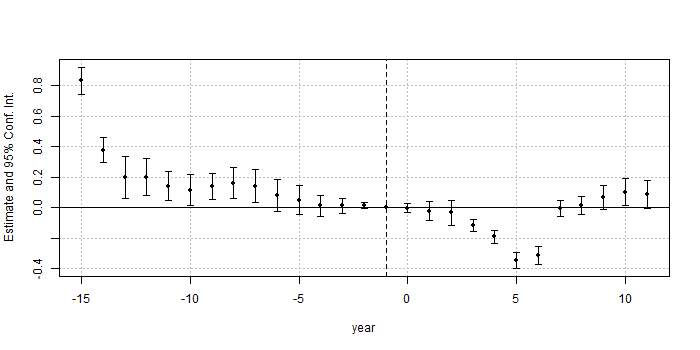
\includegraphics[width=0.85\textwidth]{violent}
	\end{center}
	\caption{Sun and Abraham Event Study - Violent Crime Rate Log}
	\label{fig:violent_graph}
\end{figure}

As shown by the figure, it is not clear the pretrend assumptions hold. Indeed, for many years prior to the treatment year, the estimated effect is statistically significantly different from zero with a 95 percent confidence interval. Additionally, we notice that we see no average treatment effect for the first few years after treatment, before a significant departure for a few years followed by a reversion.

\begin{figure}[H]
	\begin{center}
		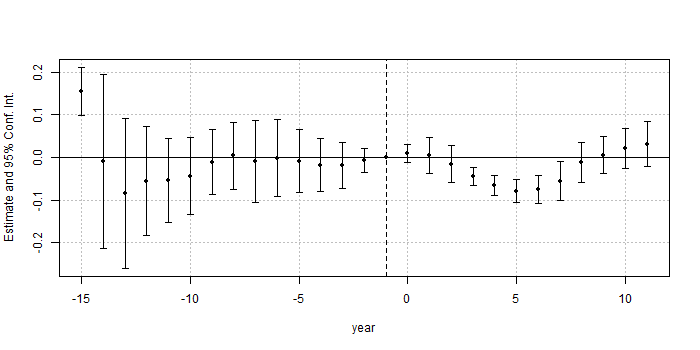
\includegraphics[width=0.85\textwidth]{property}
	\end{center}
	\caption{Sun and Abraham Event Study - Property Crime Rate Log}
	\label{fig:property_graph}
\end{figure}

For the Property Crime Rate Log variable, we see that for all but one year prior to treatment it could be that pretrend assumptions hold, though the confidence intervals appear relatively large. Similar to the prior chart, we have an interesting ``u'' shape after treatment where we see no cohort average treatment effect, some average cohort treatment effect, and no average cohort treatment effect again.

For most of the other crimes analyzed, we see similarly erratic and inconclusive shapes. In many instances the pretrend assumptions appear to hold, but not all. For instance, the Assault Crime Rate Log stands out as the pretrend assumptions do not appear to hold, and we actually see in later treatment years a \emph{positive} average treatment effect.

Please see the appendix for the Event Study figures for the other seven crime categories analyzed.

\section{Conclusion}

Through this replication and extension, we have shown four different estimators applied to the same data can yield different and interesting results. We first estimated the fixed effects model consistent with the original approach by Lott and Mustard, albeit applied to state level data rather than county level. We then dug in further to the meaning and composition of the resulting fixed effects coefficients by applying the Bacon Decomposition. Finally, we applied the Callaway and Sant'anna alternative estimator and the Sun and Abraham event study to get more specific group-timing treatment effects and assess bias associated with treatment effect heterogeneity. The application of these various approaches showed just how important estimation approach and a critical eye toward potential sources of bias is when performing independent research. Furthermore, we see how far the study of difference in difference models has come in extracting ``more true'' casual coefficients. Historically, when studying two groups with one treatment, the assumptions and validation was more straightforward. Now, however, newer more nuanced models are required to support more complex scenarios involving multiple treatment groups receiving treatment at multiple times.  

\newpage

\section{Appendix}

\subsection{Detailed Two Way Fixed Effects Tables}


\begin{table}[htbp]
   \caption{\label{tab:replicatetable3a} Replication of Table 3 Panel A : Fixed Effects Regressions}
   \centering
   \small
   \begin{tabular}{lccc}
      \tabularnewline \midrule \midrule
      Dependent Variables:     & violent\_crime\_rate\_log    & property\_crime\_rate\_log    & murder\_crime\_rate\_log\\     
      Model:                   & (1)                          & (2)                           & (3)\\  
      \midrule
      \emph{Variables}\\
      shalll                   & -0.0978$^{***}$              & -0.0072                       & -0.0507\\   
                               & (0.0324)                     & (0.0194)                      & (0.0394)\\   
      Relevant\_Arrest\_Rate   & -0.0003                      & -0.0020$^{*}$                 & -0.0004\\   
                               & (0.0004)                     & (0.0011)                      & (0.0002)\\   
      \midrule
      \emph{Fixed-effects}\\
      state                    & Yes                          & Yes                           & Yes\\  
      year                     & Yes                          & Yes                           & Yes\\  
      \midrule
      \emph{Fit statistics}\\
      Observations             & 802                          & 809                           & 806\\  
      R$^2$                    & 0.98146                      & 0.96445                       & 0.94792\\  
      Within R$^2$             & 0.47334                      & 0.55426                       & 0.31137\\  
      \midrule \midrule
      \multicolumn{4}{l}{\emph{Clustered (state) standard-errors in parentheses}}\\
      \multicolumn{4}{l}{\emph{Signif. Codes: ***: 0.01, **: 0.05, *: 0.1}}\\
   \end{tabular}
   
   \par \raggedright 
   Control variables ommited from table, 
                           though they were included in the analysis. 
                           Consistent with the original paper, 
                           control variables include: density, personal\_income\_rpc, unemployment\_insurance\_rpc, income\_maintenance\_rpc, retirement\_payments\_rpc, state\_population, ppwm1019, ppbm1019, ppnm1019, ppwf1019, ppbf1019, ppnf1019, ppwm2029, ppbm2029, ppnm2029, ppwf2029, ppbf2029, ppnf2029, ppwm3039, ppbm3039, ppnm3039, ppwf3039, ppbf3039, ppnf3039, ppwm4049, ppbm4049, ppnm4049, ppwf4049, ppbf4049, ppnf4049, ppwm5064, ppbm5064, ppnm5064, ppwf5064, ppbf5064, ppnf5064, ppwm65o, ppbm65o, ppnm65o, ppwf65o, ppbf65o, ppnf65o.
\end{table}





\begin{table}[htbp]
   \caption{\label{tab:replicatetable3b} Replication of Table 3 Panel B : Fixed Effects Regressions}
   \centering
   \small
   \begin{tabular}{lccc}
      \tabularnewline \midrule \midrule
      Dependent Variables:     & rape\_crime\_rate\_log    & assault\_crime\_rate\_log    & robbery\_crime\_rate\_log\\     
      Model:                   & (1)                       & (2)                          & (3)\\  
      \midrule
      \emph{Variables}\\
      shalll                   & -0.0340                   & -0.1004$^{**}$               & -0.0532\\   
                               & (0.0395)                  & (0.0424)                     & (0.0439)\\   
      Relevant\_Arrest\_Rate   & -0.0006                   & -0.0028$^{***}$              & -0.0014\\   
                               & (0.0005)                  & (0.0009)                     & (0.0009)\\   
      \midrule
      \emph{Fixed-effects}\\
      state                    & Yes                       & Yes                          & Yes\\  
      year                     & Yes                       & Yes                          & Yes\\  
      \midrule
      \emph{Fit statistics}\\
      Observations             & 799                       & 809                          & 808\\  
      R$^2$                    & 0.94240                   & 0.96632                      & 0.98389\\  
      Within R$^2$             & 0.52351                   & 0.51645                      & 0.50471\\  
      \midrule \midrule
      \multicolumn{4}{l}{\emph{Clustered (state) standard-errors in parentheses}}\\
      \multicolumn{4}{l}{\emph{Signif. Codes: ***: 0.01, **: 0.05, *: 0.1}}\\
   \end{tabular}
   
   \par \raggedright 
   Control variables ommited from table, 
                           though they were included in the analysis. 
                           Consistent with the original paper, 
                           control variables include: density, personal\_income\_rpc, unemployment\_insurance\_rpc, income\_maintenance\_rpc, retirement\_payments\_rpc, state\_population, ppwm1019, ppbm1019, ppnm1019, ppwf1019, ppbf1019, ppnf1019, ppwm2029, ppbm2029, ppnm2029, ppwf2029, ppbf2029, ppnf2029, ppwm3039, ppbm3039, ppnm3039, ppwf3039, ppbf3039, ppnf3039, ppwm4049, ppbm4049, ppnm4049, ppwf4049, ppbf4049, ppnf4049, ppwm5064, ppbm5064, ppnm5064, ppwf5064, ppbf5064, ppnf5064, ppwm65o, ppbm65o, ppnm65o, ppwf65o, ppbf65o, ppnf65o.
\end{table}





\begin{table}[htbp]
   \caption{\label{tab:replicatetable3c} Replication of Table 3 Panel C : Fixed Effects Regressions}
   \centering
   \small
   \begin{tabular}{lccc}
      \tabularnewline \midrule \midrule
      Dependent Variables:     & burglary\_crime\_rate\_log    & larceny\_crime\_rate\_log    & autotheft\_crime\_rate\_log\\     
      Model:                   & (1)                           & (2)                          & (3)\\  
      \midrule
      \emph{Variables}\\
      shalll                   & -0.0461$^{**}$                & 0.0033                       & -0.0090\\   
                               & (0.0190)                      & (0.0138)                     & (0.0283)\\   
      Relevant\_Arrest\_Rate   & -0.0052$^{***}$               & -0.0011                      & -0.0003$^{*}$\\   
                               & (0.0015)                      & (0.0010)                     & (0.0002)\\   
      \midrule
      \emph{Fixed-effects}\\
      state                    & Yes                           & Yes                          & Yes\\  
      year                     & Yes                           & Yes                          & Yes\\  
      \midrule
      \emph{Fit statistics}\\
      Observations             & 809                           & 809                          & 808\\  
      R$^2$                    & 0.95597                       & 0.96600                      & 0.96116\\  
      Within R$^2$             & 0.50429                       & 0.54529                      & 0.60312\\  
      \midrule \midrule
      \multicolumn{4}{l}{\emph{Heteroskedasticity-robust standard-errors in parentheses}}\\
      \multicolumn{4}{l}{\emph{Signif. Codes: ***: 0.01, **: 0.05, *: 0.1}}\\
   \end{tabular}
   
   \par \raggedright 
   Control variables ommited from table, 
                           though they were included in the analysis. 
                           Consistent with the original paper, 
                           control variables include: density, personal\_income\_rpc, unemployment\_insurance\_rpc, income\_maintenance\_rpc, retirement\_payments\_rpc, state\_population, ppwm1019, ppbm1019, ppnm1019, ppwf1019, ppbf1019, ppnf1019, ppwm2029, ppbm2029, ppnm2029, ppwf2029, ppbf2029, ppnf2029, ppwm3039, ppbm3039, ppnm3039, ppwf3039, ppbf3039, ppnf3039, ppwm4049, ppbm4049, ppnm4049, ppwf4049, ppbf4049, ppnf4049, ppwm5064, ppbm5064, ppnm5064, ppwf5064, ppbf5064, ppnf5064, ppwm65o, ppbm65o, ppnm65o, ppwf65o, ppbf65o, ppnf65o.
\end{table}




\newpage

\subsection{Additional Bacon Decomposition Tables}

\begin{table}[H]

\caption{\label{tab:tab:bacondecompositionMurder}Bacon Decomposition - Murder Crime Rate Log}
\centering
\begin{tabular}[t]{lrrr}
\toprule
Type & Average Estimate & Group Weight & Weighted Estimate\\
\midrule
\cellcolor{gray!6}{Earlier vs Later Treated} & \cellcolor{gray!6}{0.0545024} & \cellcolor{gray!6}{0.0683810} & \cellcolor{gray!6}{0.0054525}\\
Later vs Always Treated & -0.0384771 & 0.1589397 & -0.0012542\\
\cellcolor{gray!6}{Later vs Earlier Treated} & \cellcolor{gray!6}{0.0188246} & \cellcolor{gray!6}{0.0233921} & \cellcolor{gray!6}{0.0000418}\\
Treated vs Untreated & -0.0848318 & 0.7492871 & -0.0415959\\
\cellcolor{gray!6}{Total TWFE} & \cellcolor{gray!6}{NaN} & \cellcolor{gray!6}{NaN} & \cellcolor{gray!6}{-0.0373558}\\
\bottomrule
\end{tabular}
\end{table}


\begin{table}[H]

\caption{\label{tab:tab:bacondecompositionRape}Bacon Decomposition: Rape Crime Rate Log}
\centering
\begin{tabular}[t]{lrrr}
\toprule
Type & Average Estimate & Group Weight & Weighted Estimate\\
\midrule
\cellcolor{gray!6}{Earlier vs Later Treated} & \cellcolor{gray!6}{-0.0264193} & \cellcolor{gray!6}{0.0683810} & \cellcolor{gray!6}{-0.0026425}\\
Later vs Always Treated & -0.2001560 & 0.1589397 & -0.0305273\\
\cellcolor{gray!6}{Later vs Earlier Treated} & \cellcolor{gray!6}{-0.0106483} & \cellcolor{gray!6}{0.0233921} & \cellcolor{gray!6}{-0.0019283}\\
Treated vs Untreated & -0.0030557 & 0.7492871 & 0.0030423\\
\cellcolor{gray!6}{Total TWFE} & \cellcolor{gray!6}{NaN} & \cellcolor{gray!6}{NaN} & \cellcolor{gray!6}{-0.0320558}\\
\bottomrule
\end{tabular}
\end{table}


\begin{table}[H]

\caption{\label{tab:tab:bacondecompositionAssault}Bacon Decomposition - Assault Crime Rate Log}
\centering
\begin{tabular}[t]{lrrr}
\toprule
Type & Average Estimate & Group Weight & Weighted Estimate\\
\midrule
\cellcolor{gray!6}{Earlier vs Later Treated} & \cellcolor{gray!6}{0.149} & \cellcolor{gray!6}{0.068} & \cellcolor{gray!6}{0.008}\\
Later vs Always Treated & -0.031 & 0.159 & 0.001\\
\cellcolor{gray!6}{Later vs Earlier Treated} & \cellcolor{gray!6}{-0.017} & \cellcolor{gray!6}{0.023} & \cellcolor{gray!6}{-0.003}\\
Treated vs Untreated & -0.221 & 0.749 & -0.138\\
\cellcolor{gray!6}{Total TWFE} & \cellcolor{gray!6}{NaN} & \cellcolor{gray!6}{NaN} & \cellcolor{gray!6}{-0.132}\\
\bottomrule
\end{tabular}
\end{table}


\begin{table}[H]

\caption{\label{tab:tab:bacondecompositionRobbery}Bacon Decomposition - Robbery Crime Rate Log}
\centering
\begin{tabular}[t]{lrrr}
\toprule
Type & Average Estimate & Group Weight & Weighted Estimate\\
\midrule
\cellcolor{gray!6}{Earlier vs Later Treated} & \cellcolor{gray!6}{0.0961047} & \cellcolor{gray!6}{0.0683810} & \cellcolor{gray!6}{0.0073682}\\
Later vs Always Treated & 0.0940074 & 0.1589397 & 0.0174822\\
\cellcolor{gray!6}{Later vs Earlier Treated} & \cellcolor{gray!6}{0.1505417} & \cellcolor{gray!6}{0.0233921} & \cellcolor{gray!6}{0.0020947}\\
Treated vs Untreated & -0.0263060 & 0.7492871 & -0.0100514\\
\cellcolor{gray!6}{Total TWFE} & \cellcolor{gray!6}{NaN} & \cellcolor{gray!6}{NaN} & \cellcolor{gray!6}{0.0168936}\\
\bottomrule
\end{tabular}
\end{table}


\begin{table}[H]

\caption{\label{tab:tab:bacondecompositionBurglary}Bacon Decomposition - Burglary Crime Rate Log}
\centering
\begin{tabular}[t]{lrrr}
\toprule
Type & Average Estimate & Group Weight & Weighted Estimate\\
\midrule
\cellcolor{gray!6}{Earlier vs Later Treated} & \cellcolor{gray!6}{-0.015} & \cellcolor{gray!6}{0.068} & \cellcolor{gray!6}{-0.002}\\
Later vs Always Treated & 0.017 & 0.159 & 0.005\\
\cellcolor{gray!6}{Later vs Earlier Treated} & \cellcolor{gray!6}{-0.016} & \cellcolor{gray!6}{0.023} & \cellcolor{gray!6}{-0.001}\\
Treated vs Untreated & -0.007 & 0.749 & 0.006\\
\cellcolor{gray!6}{Total TWFE} & \cellcolor{gray!6}{NaN} & \cellcolor{gray!6}{NaN} & \cellcolor{gray!6}{0.008}\\
\bottomrule
\end{tabular}
\end{table}


\begin{table}[H]

\caption{\label{tab:tab:bacondecompositionLarceny}Bacon Decomposition - Larceny Crime Rate Log}
\centering
\begin{tabular}[t]{lrrr}
\toprule
Type & Average Estimate & Group Weight & Weighted Estimate\\
\midrule
\cellcolor{gray!6}{Earlier vs Later Treated} & \cellcolor{gray!6}{0.0088734} & \cellcolor{gray!6}{0.0683810} & \cellcolor{gray!6}{-0.0004160}\\
Later vs Always Treated & 0.0477985 & 0.1589397 & 0.0080003\\
\cellcolor{gray!6}{Later vs Earlier Treated} & \cellcolor{gray!6}{0.0616798} & \cellcolor{gray!6}{0.0233921} & \cellcolor{gray!6}{0.0004859}\\
Treated vs Untreated & 0.0346292 & 0.7492871 & 0.0280699\\
\cellcolor{gray!6}{Total TWFE} & \cellcolor{gray!6}{NaN} & \cellcolor{gray!6}{NaN} & \cellcolor{gray!6}{0.0361400}\\
\bottomrule
\end{tabular}
\end{table}


\begin{table}[H]

\caption{\label{tab:tab:bacondecompositionAutotheft}Bacon Decomposition - Autotheft Crime Rate Log}
\centering
\begin{tabular}[t]{lrrr}
\toprule
Type & Average Estimate & Group Weight & Weighted Estimate\\
\midrule
\cellcolor{gray!6}{Earlier vs Later Treated} & \cellcolor{gray!6}{0.089} & \cellcolor{gray!6}{0.068} & \cellcolor{gray!6}{0.006}\\
Later vs Always Treated & 0.189 & 0.159 & 0.034\\
\cellcolor{gray!6}{Later vs Earlier Treated} & \cellcolor{gray!6}{0.099} & \cellcolor{gray!6}{0.023} & \cellcolor{gray!6}{0.002}\\
Treated vs Untreated & 0.009 & 0.749 & 0.026\\
\cellcolor{gray!6}{Total TWFE} & \cellcolor{gray!6}{NaN} & \cellcolor{gray!6}{NaN} & \cellcolor{gray!6}{0.068}\\
\bottomrule
\end{tabular}
\end{table}


\newpage

\subsection{Additional Sun and Abraham Event Study Figures}

\begin{figure}[H]
	\begin{center}
		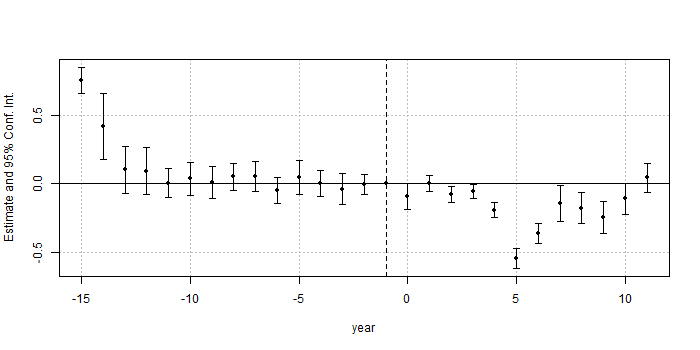
\includegraphics[width=0.85\textwidth]{murder}
	\end{center}
	\caption{Sun and Abraham Event Study - Murder Crime Rate Log}
	\label{fig:murder_graph}
\end{figure}

\begin{figure}[H]
	\begin{center}
		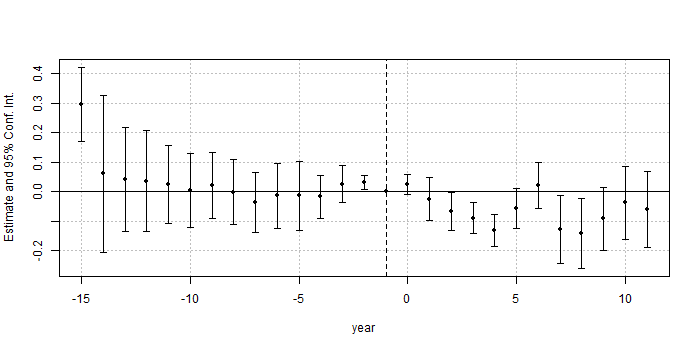
\includegraphics[width=0.85\textwidth]{rape}
	\end{center}
	\caption{Sun and Abraham Event Study - Rape Crime Rate Log}
	\label{fig:rape_graph}
\end{figure}

\begin{figure}[H]
	\begin{center}
		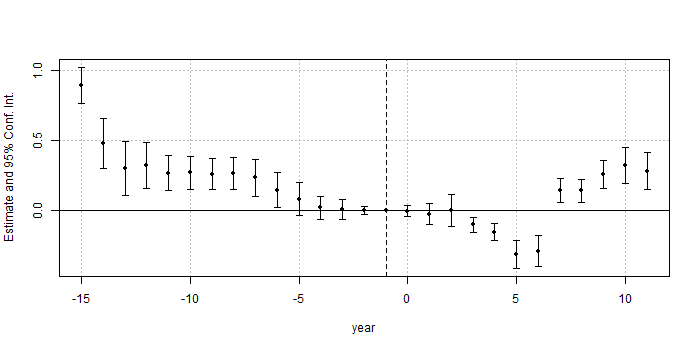
\includegraphics[width=0.85\textwidth]{assault}
	\end{center}
	\caption{Sun and Abraham Event Study - Assault Crime Rate Log}
	\label{fig:assault_graph}
\end{figure}

\begin{figure}[H]
	\begin{center}
		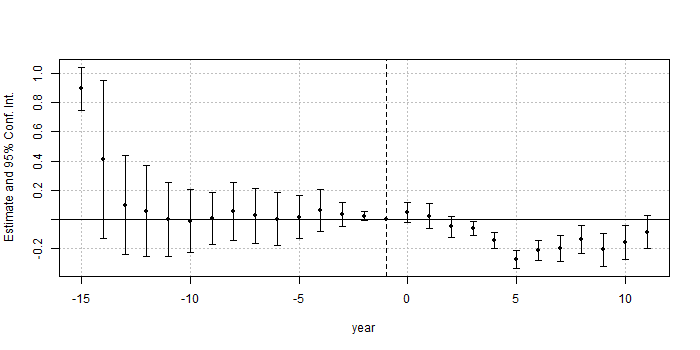
\includegraphics[width=0.85\textwidth]{robbery}
	\end{center}
	\caption{Sun and Abraham Event Study - Robbery Crime Rate Log}
	\label{fig:robbery_graph}
\end{figure}

\begin{figure}[H]
	\begin{center}
		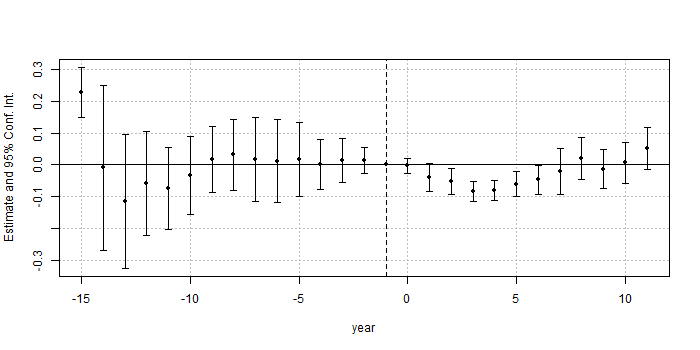
\includegraphics[width=0.85\textwidth]{burglary}
	\end{center}
	\caption{Sun and Abraham Event Study - Burglary Crime Rate Log}
	\label{fig:burglary_graph}
\end{figure}

\begin{figure}[H]
	\begin{center}
		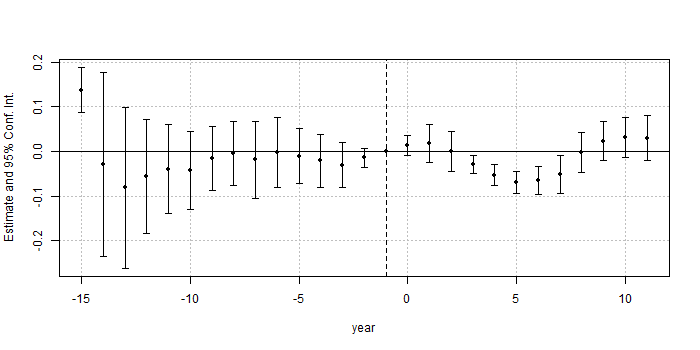
\includegraphics[width=0.85\textwidth]{larceny}
	\end{center}
	\caption{Sun and Abraham Event Study - Larceny Crime Rate Log}
	\label{fig:larceny_graph}
\end{figure}

\begin{figure}[H]
	\begin{center}
		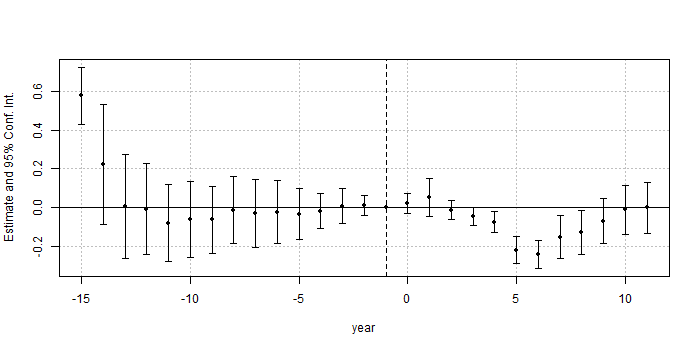
\includegraphics[width=0.85\textwidth]{autotheft}
	\end{center}
	\caption{Sun and Abraham Event Study - Auto Theft Crime Rate Log}
	\label{fig:autotheft_graph}
\end{figure}

\end{document}

